\documentclass[11pt,a4paper]{report}
\usepackage[margin=2.2cm]{geometry}
\usepackage[pdftex]{graphicx}
\usepackage{styles}
\usepackage{url} 
\usepackage[bookmarks, colorlinks=false, pdfborder={0 0 0}, pdftitle={<pdf title here>}, pdfauthor={<author's name here>}, pdfsubject={<subject here>}, pdfkeywords={<keywords here>}]{hyperref} 
\usepackage{minted}
\usepackage{tikz}
\usepackage{colortbl}
\usepackage{hyperref}
\usepackage{textcomp}
\usepackage{amssymb}
\usepackage{titlesec}
\usepackage{parskip}
\usepackage{enumitem}
\usepackage{amsmath}
\usepackage{xcolor}
\usetikzlibrary{matrix, arrows.meta, positioning, fit}
\usetikzlibrary{calc}
\usetikzlibrary{decorations.pathreplacing}

% Reduce space around sections and chapters
\titlespacing*{\chapter}{0pt}{0pt}{10pt}
\titlespacing*{\section}{0pt}{10pt}{5pt}
\titlespacing*{\subsection}{0pt}{8pt}{3pt}

% Reduce line spacing
\linespread{1.0}


\begin{document}
\renewcommand\bibname{References} 

\begin{titlepage}

\begin{center}

\textup{\small {\bf Summer Internship Project} \\ Report}\\[0.3in]

% Title
\Large \textbf {\scol{\bf Formal verification of programs with pointers }}\\[0.7in]


       

% Submitted by
\normalsize Submitted by \\[0.2in]
\scol{\textbf{Oualid CHABANE}}\\
Third year of bachelor's double degree in \\ Computer Science, Magistère d'informatique track.\\
Faculty of sciences of Orsay, university of Paris-Saclay.

\vspace{.2in}
Under the guidance of\\[0.2in]
\scol{\textbf{Arnaud Goulfouse}}\\
\scol{\textbf{Paul Patault}}\\
\scol{\textbf{Jean-Christophe Filliâtre}}\\

\vspace{.3in}

% Bottom of the page
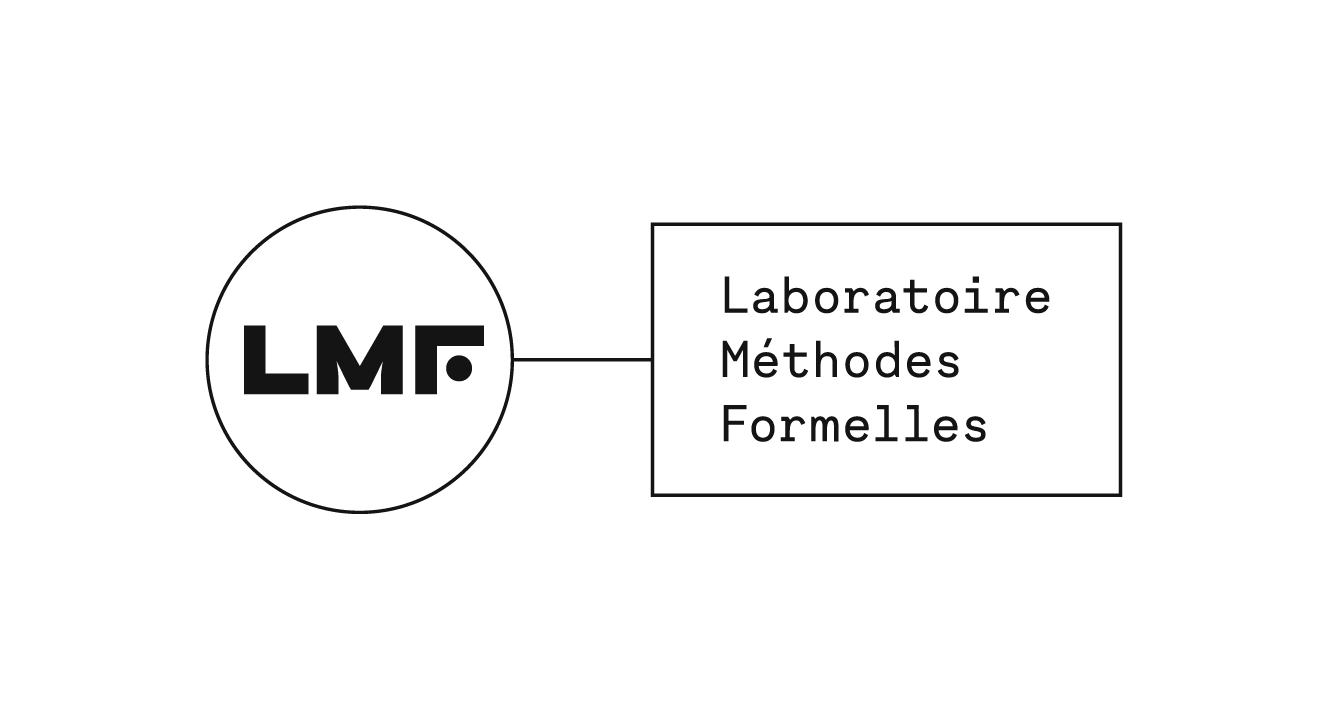
\includegraphics[width=0.5\textwidth]{lmf.png}\\[0.1in]
\Large{Department of Formal methods}\\
\normalsize
\textsc{ The Laboratoire Méthodes Formelles (LMF). }\\
4, avenue des Sciences, 91190 Gif-sur-Yvette \\
\vspace{0.2cm}
Summer Internship 2025

\end{center}

\end{titlepage}


\pagenumbering{roman}
\tableofcontents

\newpage
\pagenumbering{arabic} 

\chapter{Introduction}

\section{\scol{The Laboratoire Méthodes Formelles (LMF)}}
LMF is a joint research centre of University Paris-Saclay, CNRS, ENS Paris-Saclay, Inria, and CentraleSupélec. it's divided to multiple departments interested in various topics such as type systems, topology and quantum computing. My research project took place within \scol{Toccata's team} of the formal methods department. I worked on verification of programs with pointers under the supervision of Jean-Cristophe Filliâtre, Arnaud Golfouse and Paul Patault.

There are multiple verification tools widely used and developed at the LMF research center. Among these tools, we find Creusot and Why3.

\section{\scol{Le langage de preuve Creusot}}
\subsection{Introduction}
\textsc{Creusot} is a formal verification language used to verify \textsc{Rust} code. It checks the safety of code against compile-time errors and runtime panics, integer overflows, and, more importantly, the logical correctness of the code, ensuring it adheres to its specifications.

\textsc{Creusot} operates on top of \textsc{Why3} indirectly by translating Rust code into an intermediate verification language known as \textsc{Coma}. It facilitates the verification, and it also gives \textsc{Creusot} access to the full access to \textsc{Why3}'s features.

Below is a simple example of \textsc{Creusot} code that verifies the correctness of the \texttt{SUM\_FIRST\_N} function.

\begin{figure}[h]
\centering
\begin{minipage}{0.95\linewidth}
\begin{minted}[linenos, fontsize=\footnotesize, bgcolor=gray!5]{rust}
extern crate creusot_contracts;
use creusot_contracts::*;

#[requires(n@ * (n@ + 1) / 2 < u32::MAX@)]
#[ensures(result@ == n@ * (n@ + 1) / 2)]
pub fn sum_first_n(n: u32) -> u32 {
    let mut sum = 0;
    #[invariant(sum@ * 2 == produced.len() * (produced.len() + 1))]
    for i in 1..=n {
        sum += i;
    }
    sum
}
\end{minted}
\caption{Creusot verification example: sum of first n natural numbers}
\label{fig:sum-example}
\end{minipage}
\end{figure}

\textbf{Explanation}: 

The function \textsc{sum\_first\_n} shown above computes the sum of the first \texttt{n} natural numbers. The expressions highlighted in yellow represent its specification:
\begin{itemize}
\item \textbf{Precondition:} It asserts that the sum of the first \texttt{n} natural numbers where \texttt{n} is provided as a parameter, does not overflow the capacity of the result type. This ensures that the final sum, which will be stored in the return variable will not exceed the capacity of the return type. The operator \texttt{@} converts machine integers into mathematical integers, which are unlimited, allowing us to use arithmetic theory.
\item \textbf{Postcondition:} It states that the returned result is equal to the expected mathematical value: \texttt{n * (n + 1) / 2}
\item \textbf{Loop invariant:} The expression \texttt{produced.len()} corresponds to the number of iterations performed so far, it effectively can play the role of the loop index by applying a transformation. The reason we cannot refer directly to the loop index is due to scoping limitations.
\end{itemize}
\subsection{Ghost code in \textsc{CREUSOT}}
\textsc{Rust}'s ownership and borrowing principles make it difficult to use pointers in proofs. where the need for a notion of ghost code in such a language. Ghost code allows us to perform proofs that are not possible using only raw code and the logical world, especially when dealing with existential quantification, if we know how to construct the value we are seeking for the existential quantifier.

Recently, ghost code has been introduced in \textsc{Creusot}. The subtlety lies in the fact that ghost code is separate from the original code. Therefore, it can be safely erased at compile time, allowing only the original code and the corresponding logical formulas to be executed. This results in faster and safer proof verification. Below are some examples of how to write ghost code in \textsc{Creusot}.

\hypertarget{ghostcode}{}

\chapter{State of art}

\section{\scol{Reynolds article}}
Reynolds' article introduced a new concept in formal program verification: \emph{Separation Logic}, an extension of Hoare Logic that facilitates automatic proofs on low-level imperative programs that use shared mutable data structures, by reasoning about disjoint parts of the heap. It greatly simplifies the formalization and verification of many problems that are otherwise difficult to handle using traditional Hoare Logic, such as concurrency, memory management, and aliasing.
\\

Reynolds is particularly interested in the \hyperlink{reversal}{\texttt{in\_place\_reversal}$\dagger$} algorithm. He frequently discusses it in his research, as it is a very interesting algorithm for exploring formal proofs on mutable data structures with pointers.
\\

To prove properties of algorithms on data structures, it's usually not enough to rely only on the program's representation. We often build a logical model of the data and connect it to the program state using predicates. It's better if the logical model is inductive, because provers generally work better with inductive data structures, for instance, the intuitive logical modeling of lists are sequences, therefore we can write the following predicate to represent a list:


\begin{align}
\texttt{list}\ \epsilon\ \texttt{i} &\overset{\text{def}}{=}\ \texttt{i = nil} \\
\texttt{list}\ (a.\alpha)\ \texttt{i} &\overset{\text{def}}{=}\ \exists\ \texttt{j},\ \texttt{list}\ \alpha\ \texttt{j} \land\ \texttt{i} \hookrightarrow \texttt{a}
\end{align}


\texttt{i $\hookrightarrow$ a} means \texttt{i} points to \texttt{a}\\

We can generalize the definition of a list to list segments by passing a tuple of pointers instead of a single one. In this case, the first pointer represents the head of the sub-list, and the second pointer represents the queue of the sub-list.\\
One of key uses of separation logic can be show in case if we prohibit using \hyperlink{reversal}{\texttt{in\_place\_reversal}$\dagger$} on shared data structures, in this context, given the following precondition for in-place reversal: \texttt{list p $\alpha$}, the post-condition \texttt{list p }$\overline{\alpha}$ is not sufficient to ensure the correctness of the algorithm. consider the example in the figure below.

\begin{figure}[h!]
\centering
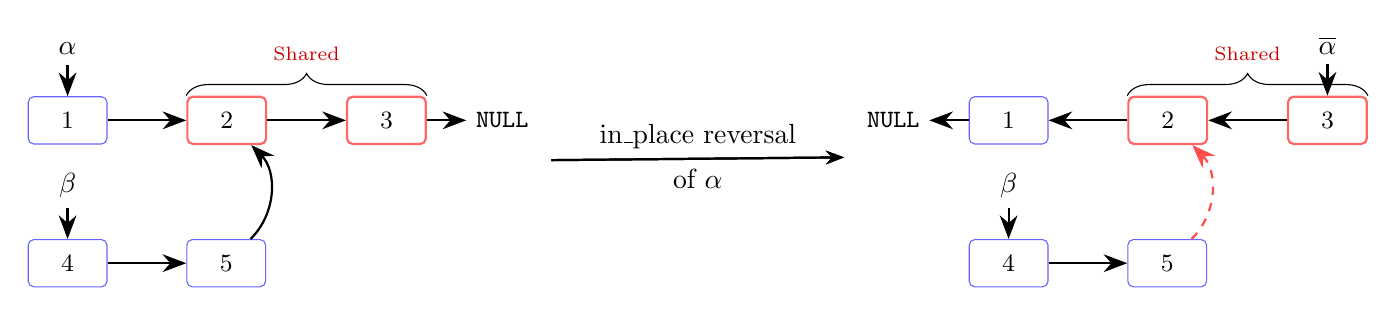
\begin{tikzpicture}[node distance=1cm and 1cm, 
    box/.style={
        rectangle, draw, minimum width=1cm, minimum height=0.6cm, rounded corners=2pt,
        font=\small, text centered
    },
    normal/.style={draw=blue!60},
    shared/.style={draw=red!60, thick},
    arrow/.style={-{Stealth[length=3mm]}, thick},
    label/.style={font=\bfseries}
]

% First diagram as a scope
\begin{scope}[local bounding box=first]
    % List A nodes
    \node[box, normal] (a1) {1};
    \node[box, shared, right=of a1] (shared3) {2};
    \node[box, shared, right=of shared3] (shared4) {3};

    % List B nodes
    \node[box, normal, below=1.2cm of a1] (b6) {4};
    \node[box, normal, right=of b6] (b7) {5};

    % List head labels
    \node[label, above=0.4cm of a1] (listA) {$\alpha$};
    \node[label, above=0.4cm of b6] (listB) {$\beta$};

    % Arrows for List A
    \draw[arrow] (listA) -- (a1);
    \draw[arrow] (a1) -- (shared3);
    \draw[arrow] (shared3) -- (shared4);

    % Arrows for List B
    \draw[arrow] (listB) -- (b6);
    \draw[arrow] (b6) -- (b7);
    \draw[arrow, bend right=45] (b7) to (shared3);

    % Null pointer
    \node[right=0.5cm of shared4, font=\small\ttfamily] (null1) {NULL};
    \draw[arrow] (shared4) -- (null1);

    % Brace for shared nodes
    \draw [decorate, decoration={brace, amplitude=8pt}]
      (shared3.north west) -- (shared4.north east) 
      node[midway, yshift=15pt, font=\scriptsize\color{red!80!black}] {Shared};
\end{scope}

% Second diagram as a scope, shifted right by 8cm (adjust as needed)
\begin{scope}[xshift=16cm, local bounding box=second]
    % List A nodes (right to left)
    \node[box, shared] (shared4b) {3};
    \node[box, shared, left=of shared4b] (shared3b) {2};
    \node[box, normal, left=of shared3b] (a1b) {1};
    
    % List B nodes
    \node[box, normal, below=1.2cm of a1b] (b6b) {4};
    \node[box, normal, right=of b6b] (b7b) {5};
    
    % List head labels
    \node[label, above=0.4cm of shared4b] (listAb) {$\overline{\alpha}$};
    \node[label, above=0.4cm of b6b] (listBb) {$\beta$};
    
    % Arrows for List A (reversed)
    \draw[arrow] (listAb) -- (shared4b);
    \draw[arrow] (shared3b) -- (a1b);
    \draw[arrow] (shared4b) -- (shared3b);
    
    % Arrows for List B
    \draw[arrow] (listBb) -- (b6b);
    \draw[arrow] (b6b) -- (b7b);
    \draw[arrow, dashed, color=red!70, bend right=45] (b7b) to (shared3b);
    
    % Null pointer at the end of the list
    \node[left=0.5cm of a1b, font=\small\ttfamily] (null1b) {NULL};
    \draw[arrow] (a1b) -- (null1b);
    
    % Brace for shared part
    \draw [decorate, decoration={brace, amplitude=8pt}]
      (shared3b.north west) -- (shared4b.north east)
      node[midway, yshift=15pt, font=\scriptsize\color{red!80!black}] {Shared};
\end{scope}
% Arrow between diagrams
\draw[->, thick, >=Stealth, shorten >=5pt, shorten <=5pt] 
  (first.east) -- node[above] {in\_place reversal} (second.west);
\draw[->, thick, >=Stealth, shorten >=5pt, shorten <=5pt] 
  (first.east) -- node[below] {of $\alpha$} (second.west);

\end{tikzpicture}

\caption{in\_place reversal on shared lists}
\label{fig:shared-lists}
\end{figure}

So we need to provide a stronger precondition that prevents such cases. One possible way is:
\[
\texttt{list\ p\ }\alpha \ \land\ \forall\,\texttt{x},\, \alpha'.\ \texttt{list\ x\ } \alpha' \rightarrow \texttt{conflicting}(\texttt{x},\ \alpha',\ \texttt{p},\ \alpha) \rightarrow \texttt{x} = \texttt{nil}
\]

where \texttt{conflicting (p: Pointer) (seq: Sequence) (p': Pointer) (seq': Sequence)} is a predicate that returns \texttt{True} if the two provided lists share any nodes. It is defined as follows:
\begin{align}
\texttt{conflicting}\ \texttt{p}\ \texttt{emp}\ \texttt{p'}\ \alpha' &\overset{\text{def}}{=} (\texttt{p} = \texttt{nil}) \\
\texttt{conflicting}\ \texttt{p}\ \alpha\ \texttt{p'}\ \texttt{emp} &\overset{\text{def}}{=} (\texttt{p'} = \texttt{nil}) \\
\texttt{conflicting}\ \texttt{p}\ (a.\alpha)\ \texttt{p'}\ (a'.\alpha') &\overset{\text{def}}{=} (\texttt{p} = \texttt{p'}) \lor {} \nonumber \\
&\quad \texttt{conflicting}\ \texttt{p}\ \alpha\ \texttt{[p'+1]}\ \alpha' \lor {} \nonumber \\
&\quad \texttt{conflicting}\ \texttt{[p+1]}\ \alpha\ \texttt{p'}\ \alpha'
\end{align}

Here, \texttt{[e]} denotes the content of the address \texttt{e}.\\
We can clearly notice that the precondition, but also the invariant, and the post-condition become extremely complicated, even more, when the program runs in a concurrent context. This is where separation logic proves invaluable. By leveraging heap separation, the specifications become significantly clearer and simpler.\\

Although \textsc{Creusot} does not support Separation Logic, its principles can be emulated through the use of the \textsc{Rust} type system and ghost code.
The latter can be used to carry over separation logic principles that are implicitly guaranteed by the \texttt{Rust} type system into the logical world. To be more precise, let us consider the interface of \texttt{PtrOwn<T>::disjoint\_lemma} as an illustrative example.

\begin{figure}[h]
\centering
\begin{minipage}{0.9\linewidth}
\begin{minted}[linenos, fontsize=\footnotesize, bgcolor=gray!5]{rust}
/// Ensures two PtrOwns reference different memory locations
#[ghost]
#[ensures(own1.ptr().addr_logic() != own2.ptr().addr_logic())]
#[ensures(*own1 == ^own1)]
pub fn disjoint_lemma(own1: &mut PtrOwn<T>, own2: &PtrOwn<T>)
\end{minted}
\caption{\texttt{PtrOwn<T>::disjoint\_lemma} interface}
\end{minipage}
\end{figure}

This lemma is admitted as an axiom in \textsc{Creusot}, and what it does is verify that the two permissions correspond to two distinct pointers on the heap.
If this lemma were logical, it would not hold, because we quantify universally over \texttt{own1} and \texttt{own2}; therefore, one could be equal to the other, and the first post-condition would not be satisfied.
However, if we admit it as a ghost lemma, the \texttt{Rust} type system, within the context of ghost code prohibits having a mutable borrow and an immutable borrow to the same value.
Therefore, \texttt{own1} and \texttt{own2} are necessarily distinct, and the validity of the axiom follows (the second post-condition is not essential for conveying the idea).

There are, however, more specialized tools designed specifically for reasoning with Separation Logic. One such tool is \textsc{Viper}, a Rust verifier that supports Separation Logic. It is built on top of \textsc{Boogie}, an intermediate verification language (IVL) developed by Microsoft Research, and is widely used in the field of formal verification. The illustration below clarifies the relationships between these languages and their connection to Separation Logic.

\begin{figure}[h]
\centering
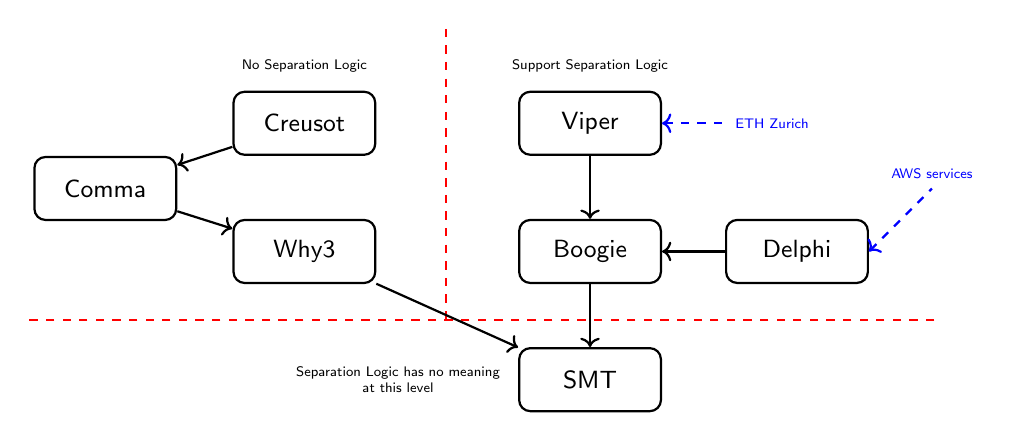
\begin{tikzpicture}[
  node distance=0.8cm and 1.8cm,
  every node/.style={font=\sffamily\small},
  box/.style={draw, rectangle, rounded corners, minimum width=1.8cm, minimum height=0.8cm, align=center},
  ->, thick
]
% Nodes
\node[box] (creusot) {Creusot};
\node[box, right=of creusot] (viper) {Viper};
\node[box, below=of viper] (boogie) {Boogie};
\node[box, left=of boogie] (why3) {Why3};
\node[box, below left=0cm and 0.7cm of creusot] (comma) {Comma};
\node[box, below=of boogie] (smt) {SMT};
\node[box, right=0.8cm of boogie] (delphi) {Delphi};

% Arrows
\draw[-, dashed, red, line width=0.8pt] 
  (1.8,1.2) -- (1.8,-2.5);

\draw[-, dashed, red, line width=0.8pt] 
  (8,-2.5) -- (-3.5,-2.5);
  
\draw (creusot) -- (comma);
\draw (comma) -- (why3);
\draw (viper) -- (boogie);
\draw (why3) -- (smt);
\draw (boogie) -- (smt);
\draw (delphi) -- (boogie);



% Arrow pointing to Delphi
\draw[<-, dashed, blue] (delphi.east) -- ++(0.8,0.8) node[above, font=\tiny\sffamily, blue] {AWS services};
\draw[<-, dashed, blue] (viper.east) -- ++(0.8,0) node[right, font=\tiny\sffamily, blue] {ETH Zurich};

% Add explanatory labels
\node[above=0.1cm of creusot, align=center, font=\tiny\sffamily] (leftlabel) 
  {No Separation Logic};
\node[above=0.1cm of viper, align=center, font=\tiny\sffamily] (rightlabel) 
  {Support Separation Logic};
\node[left=0.1cm of smt, align=center, font=\tiny\sffamily] (rightlabel) 
  {Separation Logic has no meaning\\ at this level};
\end{tikzpicture}
\caption{Illustration of the relationship between verification tools and intermediate languages.}
\label{fig:verification-diagram}
\end{figure}

\section{\scol{Different ways of implementing the problem}}
The list reversal problem has already been proven in two different ways in \textsc{Creusot}, but both methods have certain limitations:

\begin{itemize}
\item \hypertarget{BOXmeth}{\textbf{\textsc{BOX} method}}: This approach models lists using \texttt{Rust Box} type. However, it imposes strong restrictions on the memory model by prohibiting any form of sharing or aliasing, since \texttt{Box} does not support multiple references to the same memory location. As a result, the specification is simple and the proof goes through easily.
\item \hypertarget{MEMmodel}{\textbf{Memory model method}}: This approach relies on modular reasoning over the memory. In other words, it involves passing an object that models the entire memory as a parameter to each method to be verified. As a result, verification requires reasoning about the complete memory state. This can quickly lead to complex proofs even for simple algorithms. For example, suppose we have two disjoint lists in the heap, each verified using a \texttt{list} predicate. If we reverse one of them, the \texttt{list} predicate on the other is not preserved automatically, and we must explicitly include it in the proof. This makes the verification process tedious. This is where separation logic becomes useful, and the solution we propose implicitly uses its principles, thanks to \textsc{Rust} type system.
\end{itemize}

\chapter{Problem definition and proposed solution}

\section{Problem definition}

\section{Proposed solution}
\subsection{\texttt{PtrOwn} and \texttt{RawPtr}} Formally called linear algebraic types, they are used by \textsc{Creusot} to manipulate pointers in proofs. \texttt{PtrOwn} models ownership of memory cells in the ghost world and can be used in parallel with \texttt{RawPtr}, which represents the corresponding address of the cell represented by \texttt{PtrOwn}. The internal representation of \texttt{PtrOwn} is as follows:

\begin{figure}[h!]
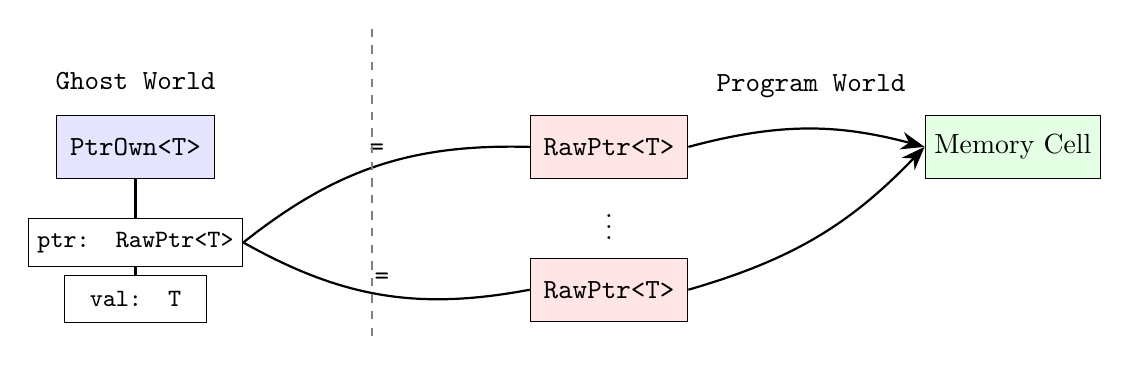
\begin{tikzpicture}[
    node distance=1cm,
    box/.style={rectangle, draw, minimum width=2cm, minimum height=0.8cm, text centered},
    field/.style={rectangle, draw, minimum width=1.8cm, minimum height=0.6cm, text centered, font=\small},
    arrow/.style={-{Stealth[length=3mm]}, thick}
]

% PtrOwn structure
\node[box, fill=blue!10] (ptrOwn) at (0,0) {\texttt{PtrOwn<T>}};

% Fields of PtrOwn
\node[field, below=0.5cm of ptrOwn] (ptrField) {\texttt{ptr: RawPtr<T>}};
\node[field, below=0.1cm of ptrField] (valField) {\texttt{val: T}};

% External RawPtr box
\node[box, fill=red!10, right=4cm of ptrOwn] (rawPtrBox) {\texttt{RawPtr<T>}};
\node[box, fill=red!10, below=1cm of rawPtrBox] (rawPtrBox2) {\texttt{RawPtr<T>}};
\node at ($(rawPtrBox)!0.5!(rawPtrBox2)$) {\vdots};


% Memory cell that RawPtr points to
\node[box, fill=green!10, right=3cm of rawPtrBox] (memoryCell) {Memory Cell};

% Arrows
% Beautiful curved arrows
\draw[thick, bend left=20] (ptrField.east) to node[midway, above] {\texttt{=}} (rawPtrBox.west);
\draw[thick, bend right=20] (ptrField.east) to  node[midway, above] {\texttt{=}} (rawPtrBox2.west);
\draw[arrow, bend left=15] (rawPtrBox.east) to (memoryCell.west);
\draw[arrow, bend right=15] (rawPtrBox2.east) to (memoryCell.west);

% Labels
\node[above=0.2cm of ptrOwn] {\texttt{Ghost World}};
\node at ($(rawPtrBox)!0.5!(memoryCell)$) [above=0.5cm] {\texttt{Program World}};


% Connecting lines for structure
\draw[thick] (ptrOwn.south) -- (ptrField.north);
\draw[thick] (ptrField.south) -- (valField.north);
% Vertical separator line
\draw[gray, thick, dashed] ($(ptrOwn.east)!0.5!(rawPtrBox.west) + (0,1.5)$) -- ($(ptrOwn.east)!0.5!(rawPtrBox.west) + (0,-2.5)$);


\end{tikzpicture}
\caption{Internal structure of \texttt{PtrOwn<T>}.}
\label{fig:ptrown-structure}
\end{figure}

Our solution relies on the use of linear algebraic types in \textsc{Creusot}, specifically, \texttt{PtrOwn} and \texttt{RawPtr}. This allows us to prove the correctness of in-place reversal even in the presence of shared data structures, making it better than the \hyperlink{BOXmeth}{BOX method$\dagger$}. Moreover, it also outperforms the \hyperlink{MEMmodel}{memory model$\dagger$} approach, our method requires to reason locally on memory. In other words, we only need to verify the parts of the heap we are manipulating, without having to reason about independent regions. This provides a form of separation logic, implicitly enforced by the Rust type system.\\
In the following we will present our solutions in steps.\\
\subsection{Data Structure}
The list type is represented by \texttt{RawPtr<Node<T>>} where \texttt{Node<T>} is defined like the following:
\begin{minted}[linenos, fontsize=\footnotesize, bgcolor=gray!5]{rust}
struct Node<T> {
    elem: T,
    pub next: RawPtr<Node<T>>,
}
\end{minted}

\subsection{Predicates}
\subsubsection{List Predicate}
\hyperlink{list}{code$\dagger$}\\
\texttt{list} predicate takes a pointer of type \texttt{RawPtr} and the abstract ghost sequence of permission \texttt{PtrOwn} that represents the list algebraically \texttt{seq}. it checks recursively that the pointers inside the permissions in the sequence correspond to the pointers in the progam world, and that the list ends with \texttt{nil}.\\
\begin{align}
    &\texttt{list p \textbf{nil} $\overset{\text{def}}{=}$ p = null\_ptr()}\\
    &\texttt{list p (a.$\alpha$) $\overset{\text{def}}{=}$ p = a.ptr() $\land$ list [p+1] $\alpha$}
\end{align}

\subsubsection{inverse Predicate}
\hyperlink{inverse}{code$\dagger$}\\
the predicate inverse takes two sequences of \texttt{PtrOwn} objects and tells if the elements of the first one are set in reverse order in the second one, on can notice that we could have written the predicated in a simpler way using the built-in function \texttt{rev}, but it is not the case, before explaining the diffrence, we show a figure of a representation of \texttt{Seq<PtrOwn<Node<T>>>} and it's corresponding list in the program world.

\begin{figure}[h]
\centering
% Option 1: Single tikzpicture with both diagrams
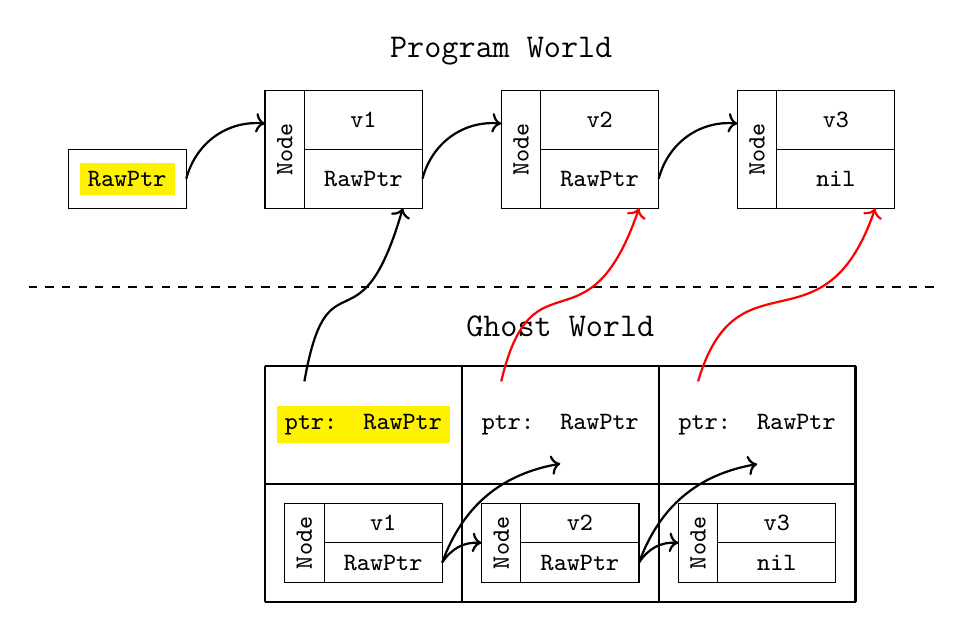
\begin{tikzpicture}
    % Program World
    \node[font=\large\bfseries] at (3,8) {\texttt{Program World}};
    
    \draw (-2.5,6) rectangle (-1,6.75);
    \node[font=\small] at (-1.75,6.375) {\texttt{\colorbox{yellow}{RawPtr}}};
    \draw[->, thick, bend left=40] (-1,6.375) to (0,7.075);
    
    % First Node
    \draw (0,6) rectangle (0.5,7.5);
    \draw (0.5,6) rectangle (2,6.75);
    \draw (0.5,6.75) rectangle (2,7.5);
    \node[rotate=90, font=\small] at (0.25,6.75) {\texttt{Node}};
    \node[font=\small] at (1.25,7.125) {\texttt{v1}};
    \node[font=\small] at (1.25,6.375) {\texttt{RawPtr}};
    
    % Arrow to second node
    \draw[->, thick, bend left=40] (2,6.375) to (3,7.075);
    
    % Second Node
    \draw (3,6) rectangle (3.5,7.5);
    \draw (3.5,6) rectangle (5,6.75);
    \draw (3.5,6.75) rectangle (5,7.5);
    \node[rotate=90, font=\small] at (3.25,6.75) {\texttt{Node}};
    \node[font=\small] at (4.25,7.125) {\texttt{v2}};
    \node[font=\small] at (4.25,6.375) {\texttt{RawPtr}};
    
    % Arrow to third node
    \draw[->, thick, bend left=40] (5,6.375) to (6,7.075);
    
    % Third Node
    \draw (6,6) rectangle (6.5,7.5);
    \draw (6.5,6) rectangle (8,6.75);
    \draw (6.5,6.75) rectangle (8,7.5);
    \node[rotate=90, font=\small] at (6.25,6.75) {\texttt{Node}};
    \node[font=\small] at (7.25,7.125) {\texttt{v3}};
    \node[font=\small] at (7.25,6.375) {\texttt{nil}};
    
    % Dashed divider line
    \draw[dashed, thick] (-3,5) -- (8.5,5);
    
    % Ghost World
    \node[font=\large\bfseries] at (3.75,4.5) {\texttt{Ghost World}};
    
    % Manual grid lines for non-uniform rows
    % Vertical lines
    \draw[black, thick] (0,1) -- (0,4);
    \draw[black, thick] (2.5,1) -- (2.5,4);
    \draw[black, thick] (5,1) -- (5,4);
    \draw[black, thick] (7.5,1) -- (7.5,4);
    
    % Horizontal lines
    \draw[black, thick] (0,1) -- (7.5,1);     % Bottom
    \draw[black, thick] (0,2.5) -- (7.5,2.5); % Middle (taller second row)
    \draw[black, thick] (0,4) -- (7.5,4);     % Top
    
    % Column 1
    % First row - ptr: RawPtr (smaller height)
    \node[font=\small] at (1.25,3.25) {\texttt{\colorbox{yellow}{ptr: RawPtr}}};
    
    % Second row - Node struct (taller height)
    \draw (0.25,1.25) rectangle (0.75,2.25);
    \draw (0.75,1.25) rectangle (2.25,1.75);
    \draw (0.75,1.75) rectangle (2.25,2.25);
    \node[rotate=90, font=\small] at (0.5,1.75) {\texttt{Node}};
    \node[font=\small] at (1.5,2) {\texttt{v1}};
    \node[font=\small] at (1.5,1.5) {\texttt{RawPtr}};
    
    % Column 2
    % First row - ptr: RawPtr
    \node[font=\small] at (3.75,3.25) {\texttt{ptr: RawPtr}};
    
    % Second row - Node struct
    \draw (2.75,1.25) rectangle (3.25,2.25);
    \draw (3.25,1.25) rectangle (4.75,1.75);
    \draw (3.25,1.75) rectangle (4.75,2.25);
    \node[rotate=90, font=\small] at (3,1.75) {\texttt{Node}};
    \node[font=\small] at (4,2) {\texttt{v2}};
    \node[font=\small] at (4,1.5) {\texttt{RawPtr}};
    
    % Column 3
    % First row - ptr: RawPtr
    \node[font=\small] at (6.25,3.25) {\texttt{ptr: RawPtr}};
    
    % Second row - Node struct
    \draw (5.25,1.25) rectangle (5.75,2.25);
    \draw (5.75,1.25) rectangle (7.25,1.75);
    \draw (5.75,1.75) rectangle (7.25,2.25);
    \node[rotate=90, font=\small] at (5.5,1.75) {\texttt{Node}};
    \node[font=\small] at (6.5,2) {\texttt{v3}};
    \node[font=\small] at (6.5,1.5) {\texttt{nil}};
    
    Cross-reference arrows from Ghost World to Program World
    From Ghost World ptr fields to Program World RawPtr elements

    \draw[->, thick]
      (0.5,3.8)
      .. controls (0.8,5.5) and (1.2,4.1)
      .. (1.75,6);
    
    \draw[->, thick, red]
      (3,3.8)
      .. controls (3.4,5.5) and (4.1,4.1)
      .. (4.75,6);
    
    \draw[->, thick, red]
      (5.5,3.8)
      .. controls (6,5.5) and (7.1,4.1)
      .. (7.75,6);
    
    % Internal Ghost World arrows (within the grid)
    \draw[->, thick, bend left=30] (2.25,1.5) to (2.75,1.75);
    \draw[->, thick, bend left=30] (4.75,1.5) to (5.25,1.75);
    \draw[->, thick, bend left=30] (2.25,1.5) to (3.75,2.755);

    
    % Arrow from second node's RawPtr to third node
    \draw[->, thick, bend left=30] (4.75,1.5) to (6.25,2.75);
    
\end{tikzpicture}


\caption{Program representation: Raw pointer-based list}
\end{figure}




% \subsection{Empty List Constructor}
% \begin{lstlisting}
% #[ensures(Self::list(result.0, *result.1))]
% #[ensures(result.0.is_null_logic())]
% pub fn empty() -> (RawPtr<Self>, Ghost<Seq<PtrOwn<Node<T>>>>)
% \end{lstlisting}
% \textbf{Purpose}: Creates an empty list represented by a null pointer and an empty permission sequence.
% \textbf{Postconditions}: Ensures the returned pointer is null and satisfies the list predicate with an empty sequence.
% \subsection{Cons Operation}
% \begin{lstlisting}
% #[requires(Self::list(l, **seq))]
% #[ensures(Self::list(result, *^seq))]
% #[ensures(forall<i:Int> 0 <= i && i < (^seq).tail().len()
% ==> seq[i] == (^seq).tail()[i])]
% #[ensures((^seq)[0].val().elem == e)]
% #[ensures((^seq)[0].ptr() == result)]
% #[ensures((^seq).len() == seq.len() + 1)]
% pub fn cons(e: T, l: RawPtr<Self>,
% seq: &mut Ghost<Seq<PtrOwn<Node<T>>>>) -> RawPtr<Self>
% \end{lstlisting}
% \textbf{Purpose}: Adds a new element to the front of the list.
% \textbf{Preconditions}: Requires that the input pointer and sequence satisfy the list predicate.
% \textbf{Postconditions}: Ensures the result forms a valid list with the new element at the front, maintaining the original elements in their relative order.
% \section{Helper Functions}
% \subsection{List Access}
% \begin{lstlisting}
% #[requires(Self::list(p, **seq))]
% #[requires(0 <= nth@ && nth@ < seq.len())]
% #[ensures(seq[nth@].val().elem == *result)]
% pub fn nth(mut p: RawPtr<Self>, nth: i128,
% seq: &Ghost<Seq<PtrOwn<Node<T>>>>) -> &T
% \end{lstlisting}
% \textbf{Purpose}: Provides safe access to the $n$-th element of the list.
% \textbf{Preconditions}: Requires a valid list and that the index is within bounds.
% \textbf{Postconditions}: Ensures the returned reference points to the element at the specified logical position.
% \subsection{In-Place Reversal}
% \begin{lstlisting}
% #[requires(Self::list(p, **seq))]
% #[ensures(Self::list(result, *^seq))]
% #[ensures(seq.len() == (^seq).len() &&
% Self::reverse(**seq, *^seq, 0, seq.len()))]
% pub fn reverse_in_place(mut p: RawPtr<Self>,
% seq: &mut Ghost<Seq<PtrOwn<Node<T>>>>) -> RawPtr<Self>
% \end{lstlisting}
% \textbf{Purpose}: Reverses the list in-place by manipulating pointer links.
% \textbf{Preconditions}: Requires a valid list representation.
% \textbf{Postconditions}: Ensures the result is a valid list with the same length, where the final sequence is the reverse of the original sequence.
% \subsection{Vector Conversion}
% \begin{lstlisting}
% #[ensures(Node::list(result.0, *result.1))]
% #[ensures(result.1.len() == vec.view().len())]
% #[ensures(forall<i: Int> 0 <= i && i < vec.view().len()
% ==> (*result.1)[i].val().elem == vec.view()[i])]
% pub fn list_of_vector1<T>(mut vec: Vec<T>)
% -> (RawPtr<Node<T>>, Ghost<Seq<PtrOwn<Node<T>>>>)
% \end{lstlisting}
% \textbf{Purpose}: Converts a vector into a linked list representation.
% \textbf{Postconditions}: Ensures the resulting list has the same length as the original vector and maintains element correspondence at each position.
% \section{Verification Approach}
% The implementation employs several key verification techniques:
% \begin{enumerate}
% \item \textbf{Ghost State}: Uses ghost sequences to maintain logical representations alongside physical pointer structures.
% \item \textbf{Loop Invariants}: Maintains complex invariants during iterative operations, particularly in the reversal algorithm.
% \item \textbf{Ownership Tracking}: Leverages Creusot's ownership system to ensure memory safety without garbage collection.
% \item \textbf{Quantified Specifications}: Uses first-order logic with quantifiers to express properties over sequences.
% \end{enumerate}


\chapter{Conclusion and prespectives}


\section{Appendix}

\hypertarget{reversal}{\subsection{\scol{\texttt{in\_place\_reversal} algorithm}}}
\begin{align*}
&\texttt{j := nil; while i } \texttt{<>} \texttt{ nil do} \\
&\quad \quad \texttt{(k := [i + 1]; [i + 1] := j; j := i; i := k).}
\end{align*}
\subsection{\scol{Code}}
\begin{minted}[breaklines=true]{rust}
extern crate creusot_contracts;
use ::std::ptr;
use creusot_contracts::ptr_own::{PtrOwn, RawPtr};
use creusot_contracts::*;
pub struct Node<T> {
    elem: T,
    pub next: RawPtr<Node<T>>,
}

impl<T> Node<T> {
    #[predicate]
    #[variant(perm_seq.len())]
    fn list(l: RawPtr<Self>, perm_seq: Seq<PtrOwn<Node<T>>>) -> bool {
        pearlite! {
            if l.is_null_logic() {
                perm_seq.len() == 0
            } else {
                 if perm_seq.len() > 0 {
                    let ptr = perm_seq[0].ptr();
                    l == ptr && Self::list(perm_seq[0].val().next, perm_seq.tail())
                } else {
                    false
                }
            }
        }
    }

    #[ensures(Self::list(result.0, *result.1))]
    #[ensures(result.0.is_null_logic())]
    pub fn empty() -> (RawPtr<Self>, Ghost<Seq<PtrOwn<Node<T>>>>) {
        (ptr::null(), Seq::new())
    }

    #[requires(Self::list(l, **seq))]
    #[ensures(Self::list(result,  *^seq))]
    #[ensures(forall<i:Int> 0 <= i && i < (^seq).tail().len() ==> seq[i] == (^seq).tail()[i])]
    #[ensures((^seq)[0].val().elem == e)]
    #[ensures((^seq)[0].ptr() == result)]
    #[ensures((^seq).len() == seq.len() + 1)]
    pub fn cons(e: T, l: RawPtr<Self>, seq: &mut Ghost<Seq<PtrOwn<Node<T>>>>) -> RawPtr<Self> {
        let (raw, own) = PtrOwn::new(Node { elem: e, next: l });

        let _seq2 = snapshot!(**seq);
        ghost!(seq.push_front_ghost(own.into_inner()));
        proof_assert!(*_seq2 == seq.tail());

        raw
    }

    #[requires(Self::list(p, **seq))]
    #[requires(0 <= nth@ && nth@ < seq.len() )]
    #[ensures(seq[nth@].val().elem == *result)]
    pub fn nth(mut p: RawPtr<Self>, nth: i128, seq: &Ghost<Seq<PtrOwn<Node<T>>>>) -> &T {
        let mut i = 0;
        proof_assert!(**seq == seq.subsequence(0, seq.len()));
        #[invariant(0 <= i@ && i@ <= nth@)]
        #[invariant(Self::list(p, seq.subsequence(i@, seq.len())))]
        loop {
            let rw = unsafe {
                PtrOwn::as_ref(p, ghost!(seq.get_ghost(Int::new(i).into_inner()).unwrap()))
            };

            if i == nth {
                return &rw.elem;
            }

            p = rw.next;
            proof_assert!(seq.subsequence(i@, seq.len()).tail() == seq.subsequence(i@+1, seq.len()));
            i += 1;
        }
    }

    #[predicate]
    pub fn inverse(seq: Seq<PtrOwn<Node<T>>>, other: Seq<PtrOwn<Node<T>>>, lb: Int, lh: Int) -> bool
    where
        T: Sized,
    {
        pearlite! {
             forall<i: Int>
            lb <= i && i < lh
            ==> seq[i].val().elem == other[other.len() - i - 1].val().elem
        }
    }

    #[requires(Self::list(p, **seq))]
    #[ensures(Self::list(result, *^seq))]
    #[ensures(seq.len() == (^seq).len())]
    #[ensures(Self::inverse(**seq, *^seq, 0, (*^seq).len()))]
    pub fn reverse_in_place(
        mut p: RawPtr<Self>,
        seq: &mut Ghost<Seq<PtrOwn<Node<T>>>>,
    ) -> RawPtr<Self> {
        snapshot! {
            let _ = Seq::<T>::ext_eq;
        };
        let mut q: *const Node<T> = ptr::null();
        let mut reverted_seq = Seq::new();
        let _seq0 = snapshot!(**seq);

        #[invariant(Self::list(q, *reverted_seq))]
        #[invariant(Self::list(p, **seq))]
        #[invariant(Self::inverse(_seq0.subsequence(0, reverted_seq.len()), *reverted_seq, 0, reverted_seq.len()))]
        #[invariant(reverted_seq.len() + seq.len() == _seq0.len())]
        #[invariant(**seq == _seq0.subsequence(reverted_seq.len(), _seq0.len()))]
        #[invariant(inv(seq))]
        #[invariant(inv(reverted_seq))]
        while !p.is_null() {
            let _sloop_entry = snapshot!(**seq);
            let _revs_loop_entry = snapshot!(*reverted_seq);
            let p2 =
                unsafe { PtrOwn::as_mut(p, ghost!(seq.get_mut_ghost(*ghost!(0int)).unwrap())) };
            let next = p2.next;
            p2.next = q;
            q = p;
            p = next;
            let _sloop_exit = snapshot!(**seq);

            ghost!((*reverted_seq).push_front_ghost(seq.pop_front_ghost().unwrap()));

            //a0156: Assertion used to prove invariant #1 (we can remove it and use use_th seq.FreeMonoid instead)
            proof_assert!(reverted_seq.tail() == *_revs_loop_entry);

            //Hypothesis: invariant(Self::list (p, **seq))
            // We need to add to the hypothesis the fac that the tail of the previous seq is the new seq
            //a1369
            proof_assert!((*_sloop_exit).tail() == **seq);

            //In order to proof the last assertion, we need the following assertion
            //It esnures that seq.tail() didn't change between the beginig of the loop and the end, what ensures the stability of our invariant
            //a7070
            proof_assert!((*_sloop_exit).tail() == (*_sloop_entry).tail());

            //this should be enough to prove #[invariant(Self::list (p, **seq))], whith using the latter, creusot proves well the remaining invariant about q
            //proof_assert!(Self::list(p, (*snap2).tail()));
            //a1313
            proof_assert!(Self::list(p, (*_sloop_exit).tail()));
            // ==> invariant #1 checks for iteration n+1
        }
        //Pour montrer ensures#1 (ensures(seq.len() == (^seq).len() && Self::inverse(**seq, *^seq, 0, seq.len())))
        //a4224
        proof_assert!(_seq0.subsequence(0, reverted_seq.len()) == *_seq0);
        ghost!(**seq = reverted_seq.into_inner());
        q
    }
}

#[ensures(Node::list(result.0, *result.1))]
#[ensures(result.1.len() == vec.view().len())]
#[ensures(forall<i: Int> 0 <= i && i < vec.view().len() ==> (*result.1)[i].val().elem == vec.view()[i])]
pub fn list_of_vector1<T>(mut vec: Vec<T>) -> (RawPtr<Node<T>>, Ghost<Seq<PtrOwn<Node<T>>>>) {
    //Takes possession of elements in the vector
    let (mut l, mut seq) = Node::empty();
    let _vec0 = snapshot!(vec);
    #[invariant(forall<i: Int>
        vec.view().len() <= i && i < _vec0.view().len() ==> seq[i - vec.view().len()].val().elem == _vec0.view()[i])]
    #[invariant(Node::list(l, *seq))]
    #[invariant(vec.view().len() + seq.len() == _vec0.view().len())]
    #[invariant(forall<i: Int> 0 <= i && i < vec.view().len() ==> vec.view()[i] == _vec0.view()[i])]
    #[invariant(inv(seq))]
    loop {
        if let Some(v) = vec.pop() {
            l = Node::cons(v, l, &mut seq);
        } else {
            break;
        }
    }
    (l, seq)
}

pub fn tr() {
    let v1 = creusot_contracts::vec![1, 5, 3];
    let (list1, mut _seq1) = list_of_vector1(v1.clone());
    assert!(*Node::nth(list1, 0, &_seq1) == 1);
    assert!(*Node::nth(list1, 1, &_seq1) == 5);
    assert!(*Node::nth(list1, 2, &_seq1) == 3);
    let l2 = Node::reverse_in_place(list1, &mut _seq1);
    assert!(*Node::nth(l2, 2, &_seq1) == 1);
    assert!(*Node::nth(l2, 1, &_seq1) == 5);
    assert!(*Node::nth(l2, 0, &_seq1) == 3);

    print!("ok");
}
\end{minted}


\end{document}